\chapter{Formulario T-18: Propuesta de implantación y puesta en marcha controlada}

Este formulario presenta la propuesta de implantación y puesta en marcha controlada que exige el Formulario T-18 de las Bases Administrativas. Cubre por separado la Etapa 1 (marcha blanca de los meses 13 a 15 y producción desde el mes 16) y la Etapa 2 (marcha blanca de los meses 19 y 20 y producción desde el mes 21), el plan de convivencia entre ambas y el procedimiento de reversión. El Subdocumento 7, sección 7.3, resume y analiza esta propuesta.

La propuesta aplica las siete condiciones que el Caso 02 impone a toda estrategia de puesta en producción (sección 13.3), responde los nueve puntos de la sección 17.6 y cumple los requisitos RT-20.01 a RT-20.08 de las Bases Técnicas Transversales. La secuencia de olas, el criterio de avance, la dotación de estabilización y la medición de la adopción son los declarados en el Capítulo 3, sección 3.4.4. La estrategia técnica de despliegue es la del Capítulo 4, apartado 4.2.4.1.2 «Liberación y reversión», con único escritor y olas conforme al apartado 4.1.8, y los paquetes de trabajo citados son los de la EDT del Formulario T-14.

\section{Reglas comunes de implantación}

Las dos etapas siguen las mismas ocho reglas, y cada una responde a una condición del caso o de las Bases:

\begin{itemize}
\item \textbf{Convivencia antes del cambio.} Nada entra en producción sin haber convivido con la forma actual de trabajar durante su marcha blanca, con conciliación diaria y posibilidad de volver atrás (Caso 02, sección 13.3, condición 1; RT-20.03).

\item \textbf{Fechas prohibidas.} Ningún despliegue, paso a producción, inicio de ola ni corte de datos ocurre durante todo septiembre, durante diciembre ni en los tres primeros días hábiles de cada mes (Capítulo 4, Tabla 14, apartado 4.2.4.1.4). Del 1 al 25 de septiembre no se interviene ningún sistema (Caso 02, RT-10.05).

\item \textbf{Olas, no un evento único.} El despliegue avanza por proceso, por sitio y por zona comercial, y nunca afecta a la vez a la bodega, la preventa, el reparto y la facturación (condición 3; RT-20.01).

\item \textbf{Ventana de despacho protegida.} No se despliega durante la ventana de 05:30 a 07:00, que no admite indisponibilidad (RT-10.05 del caso). Las intervenciones en bodega se programan y acompañan en el turno de noche, de 22:00 a 06:00 (condición 4).

\item \textbf{Despliegue azul-verde con indicadores de funcionalidad (feature flags).} Cada capacidad nueva se publica en un entorno paralelo y se habilita por sitio y por ola mediante indicadores de funcionalidad, de modo que la reversión técnica consiste en volver a la entrega previa por azul-verde/canario o desactivar el indicador (Capítulo 4, apartado 4.2.4.1.2). Cada operación tiene un único escritor autorizado: no se habilita doble escritura de stock, cobros ni guías de despacho (Capítulo 4, apartado 4.1.8).

\item \textbf{Reversión en dos niveles.} El nivel técnico vuelve a la entrega previa mediante azul-verde/canario o desactiva el indicador de funcionalidad. El operacional conserva o restituye la versión operativa local probada con un único escritor; lo ordena Operaciones del CLIENTE y debe completarse antes de las 05:30. Papel y consultas son apoyo, no sustitución manual del despacho crítico. Los registros capturados permanecen en cola y se concilian al retomar (Capítulo 3, sección 3.4.4; RT-20.02).

\item \textbf{Estabilización declarada.} Cada paso a producción tiene una estabilización de cuatro semanas por ola, con la dotación declarada en la sección 2.6 y sin costo adicional (condición 7; RT-20.05 y RT-20.06).

\item \textbf{Definición de terminado y aceptación.} Ningún entregable de implantación se da por terminado sin código, pruebas, documentación, seguridad y despliegue verificados (RT-20.07). Cada hito se acepta con un protocolo de criterios objetivos y verificables, firmado por la Contraparte Técnica (RT-20.08; Bases Administrativas, Art. 18.1).

\end{itemize}
\section{Etapa 1: marcha blanca de los meses 13 a 15 y producción desde el mes 16}

La Etapa 1 pone en producción la mayor parte del alcance y incluye verificaciones de catorce de los dieciséis resultados de aceptación del caso; por eso su implantación se describe con más detalle que la de la Etapa 2.

\subsection{Alcance y olas}

La Etapa 1 pone en producción la trazabilidad de recepción, la bodega con FEFO y la preparación nocturna, la cadena de frío, la preventa sin conexión, la planificación de rutas, el reparto con prueba de entrega digital, las devoluciones y envases, la rendición y los indicadores operacionales: los módulos M1 a M10 y M12 (paquetes 3.4.1 a 3.4.11 del Formulario T-14). La implantación sigue el orden de las dependencias de datos en tres olas (Capítulo 3, sección 3.4.4; paquete 4.1.1), como presenta la Tabla \ref{tab:T18-olas}.

\parte{tablas/tab_T18_olas}

El calendario de olas respeta los meses 13–15, pero su cierre se calcula con fechas reales. Sea F el instante final de la marcha blanca: el 100 \% del alcance debe estar operativo antes de F − 28 días y sostener volumen real e indicadores durante [F − 28 días, F). Cada activación debe respetar 1–25 de septiembre, todo diciembre y los primeros tres días hábiles del mes; también evita 05:30–07:00 y no detiene rutas. La secuencia vigente de §6.1 adelanta los remanentes a semana 8, subordinada a ese límite. Un retraso exige replanificar antes de H6; no se recorta la evidencia ni se desplazan automáticamente las fases siguientes.

\begin{figure}[htbp]
  \centering
  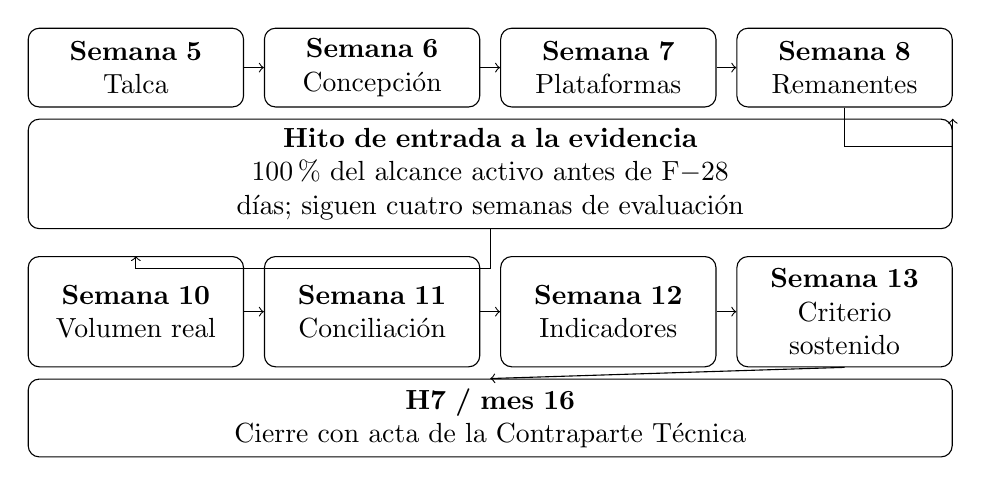
\begin{tikzpicture}[font=\LFXcuerpofigura]
    \node[draw,rounded corners,align=center,text width=2.5cm,minimum height=10mm]
      (w5) at (0,0) {\textbf{Semana 5}\\Talca};
    \node[draw,rounded corners,align=center,text width=2.5cm,minimum height=10mm]
      (w6) at (3,0) {\textbf{Semana 6}\\Concepción};
    \node[draw,rounded corners,align=center,text width=2.5cm,minimum height=10mm]
      (w7) at (6,0) {\textbf{Semana 7}\\Plataformas};
    \node[draw,rounded corners,align=center,text width=2.5cm,minimum height=10mm]
      (w8) at (9,0) {\textbf{Semana 8}\\Remanentes};
    \draw[->] (w5) -- (w6);
    \draw[->] (w6) -- (w7);
    \draw[->] (w7) -- (w8);
    \node[draw,rounded corners,align=center,text width=11.5cm,minimum height=11mm]
      (gate) at (4.5,-1.35)
      {\textbf{Hito de entrada a la evidencia}\\
       100\,\% del alcance activo antes de F$-$28 días; siguen cuatro semanas de evaluación};
    \draw[->] (w8.south) -- ++(0,-5mm) -| (gate.north east);
    \node[draw,rounded corners,align=center,text width=2.5cm,minimum height=14mm]
      (d1) at (0,-3.1) {\textbf{Semana 10}\\Volumen real};
    \node[draw,rounded corners,align=center,text width=2.5cm,minimum height=14mm]
      (d2) at (3,-3.1) {\textbf{Semana 11}\\Conciliación};
    \node[draw,rounded corners,align=center,text width=2.5cm,minimum height=14mm]
      (d3) at (6,-3.1) {\textbf{Semana 12}\\Indicadores};
    \node[draw,rounded corners,align=center,text width=2.5cm,minimum height=14mm]
      (d4) at (9,-3.1) {\textbf{Semana 13}\\Criterio sostenido};
    \draw[->] (gate.south) -- ++(0,-5mm) -| (d1.north);
    \draw[->] (d1) -- (d2);
    \draw[->] (d2) -- (d3);
    \draw[->] (d3) -- (d4);
    \node[draw,rounded corners,align=center,text width=11.5cm,minimum height=9mm]
      (h7) at (4.5,-4.45)
      {\textbf{H7 / mes 16}\\Cierre con acta de la Contraparte Técnica};
    \draw[->] (d4.south) -- (h7.north);
  \end{tikzpicture}
  \caption{Olas de la Etapa 1 durante la marcha blanca. Fuente: elaboración propia a partir del Capítulo 3, sección 3.4.4.}
  \label{fig:T18-olas}
\end{figure}

La figura presenta la secuencia de las tres olas y la acumulación de evidencia por dominio. La sección 6.1 programa las activaciones hasta la semana 8, sujetas a fechas permitidas y al límite F − 28 días. Los períodos de evidencia se superponen por dominios sin doble escritura.

\subsection{Pruebas previas a la marcha blanca y al paso a producción}

Antes de cada paso a producción se aprueban las pruebas del numeral 20.1 de las Bases Técnicas Transversales, y su cumplimiento forma parte de la certificación de la Etapa 1 (H5, mes 12; paquete 3.8.7). La Tabla \ref{tab:T18-pruebas} presenta cada prueba con su criterio de éxito.

\parte{tablas/tab_T18_pruebas}

Las pruebas cubren los tres riesgos que el caso hace críticos: la operación sin señal, el peak de septiembre y la recuperación ante desastres. La reversión operacional se ensaya además en Preproducción antes de cada corte (Capítulo 3, sección 3.4.4).

\subsection{Convivencia con la operación vigente y conciliación diaria}

Mientras dura la marcha blanca, la solución convive con la forma actual de trabajar: en bodega, con la hoja de picking impresa; en ruta, con la guía en papel; y en Talca, con el WMS de 2013 en solo lectura como respaldo de consulta hasta el cierre de la marcha blanca del sitio (supuesto S-14). En cada ola se declara cuál es el registro oficial.

Cada día se concilian ambos registros por dominio: documentos, lotes, stock, entregas y cobros. Toda diferencia se clasifica y se explica antes del cierre del día. El papel se retira en cada ola cuando cumple su criterio durante cuatro semanas consecutivas a volumen real (Capítulo 3, sección 3.4.4; RT-20.03; paquete 4.2.1).

\subsection{Indicadores diarios y umbrales de cierre}

La segunda condición del Art. 17.3 exige alcanzar «el volumen de operación real comprometido en el plan de implantación» durante al menos las cuatro últimas semanas. LafroX compromete la operación real completa de cada proceso de la ola, no una muestra ni un grupo piloto. La Tabla \ref{tab:T18-volumen} expresa ese volumen con las cifras del caso.

\parte{tablas/tab_T18_volumen}

El compromiso es que el 100 \% del volumen de cada proceso se registre en la solución durante las cuatro últimas semanas, con los demás indicadores en su umbral. Se registra el 100 \% de la operación efectivamente generada cada día, incluido su aumento durante el peak; no se exige generar pedidos artificiales ni mantener 2.600 entregas todos los días del período. Los ensayos previos verifican separadamente 1,5 veces la carga peak aplicable. Una ola que cubre una sola zona compromete el volumen de esa zona hasta que entran las demás; al cierre de la marcha blanca, todas las zonas están dentro.

Los indicadores se miden y publican cada día con el umbral que exige el Art. 17.3 para cerrar la marcha blanca (RT-20.04), como presenta la Tabla \ref{tab:T18-indicadores}.

\parte{tablas/tab_T18_indicadores}

La sexta condición es el acta de aceptación firmada por la Contraparte Técnica (paquete 4.2.3, H7). Los resultados del capítulo 18 del caso que se verifican en esta marcha blanca (R18-01 a R18-03, R18-05 a R18-10 y R18-14 a R18-16) se miden con el método y el período del Capítulo 3, Anexo 3.J. La Figura \ref{fig:T18-ciclo} resume el ciclo diario y las condiciones de cierre.

\begin{figure}[htbp]
  \centering
  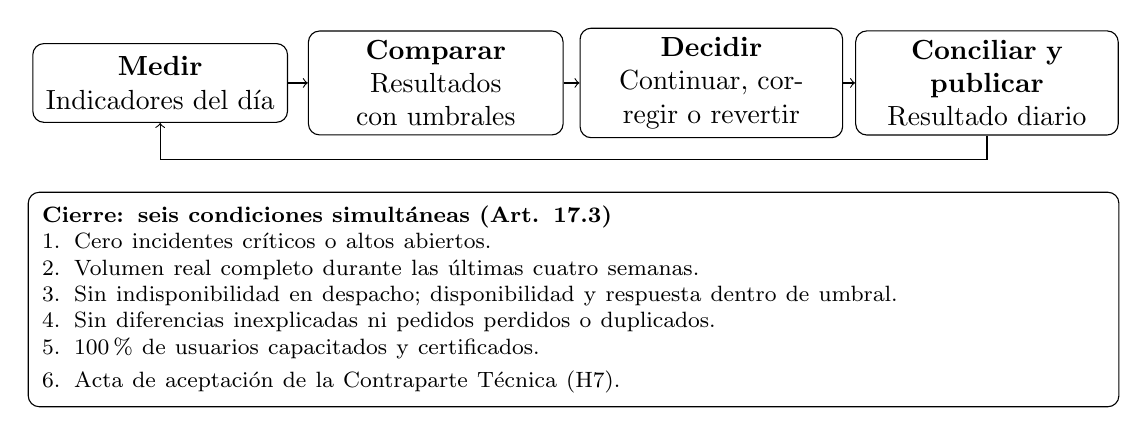
\begin{tikzpicture}[font=\LFXcuerpofigura]
    \node[draw,rounded corners,align=center,text width=3cm,minimum height=10mm]
      (measure) at (0,0)
      {\textbf{Medir}\\Indicadores del día};
    \node[draw,rounded corners,align=center,text width=3cm,minimum height=10mm]
      (compare) at (3.5,0)
      {\textbf{Comparar}\\Resultados con umbrales};
    \node[draw,rounded corners,align=center,text width=3.1cm,minimum height=10mm]
      (act) at (7,0)
      {\textbf{Decidir}\\Continuar, corregir o revertir};
    \node[draw,rounded corners,align=center,text width=3.1cm,minimum height=10mm]
      (publish) at (10.5,0)
      {\textbf{Conciliar y publicar}\\Resultado diario};
    \draw[->] (measure) -- (compare);
    \draw[->] (compare) -- (act);
    \draw[->] (act) -- (publish);
    \draw[->] (publish.south) -- ++(0,-3mm) -| (measure.south);
    \node[draw,rounded corners,align=left,text width=13.5cm,inner sep=5pt]
      at (5.25,-2.75)
      {\fontsize{8pt}{9.5pt}\selectfont
       \textbf{Cierre: seis condiciones simultáneas (Art. 17.3)}\\
       1. Cero incidentes críticos o altos abiertos.\\
       2. Volumen real completo durante las últimas cuatro semanas.\\
       3. Sin indisponibilidad en despacho; disponibilidad y respuesta dentro de umbral.\\
       4. Sin diferencias inexplicadas ni pedidos perdidos o duplicados.\\
       5. 100\,\% de usuarios capacitados y certificados.\\
       6. Acta de aceptación de la Contraparte Técnica (H7).};
  \end{tikzpicture}
  \caption{Ciclo diario de la marcha blanca y condiciones de cierre del Art. 17.3. Fuente: elaboración propia a partir de las Bases Administrativas, Art. 17.3, y del RT-20.04.}
  \label{fig:T18-ciclo}
\end{figure}

Cada día se decide entre continuar, corregir o revertir, y la marcha blanca cierra solo cuando las seis condiciones se cumplen a la vez.

\subsection{Procedimiento de reversión}

La reversión la autoriza el responsable de operaciones del CLIENTE cuando un indicador amenaza el despacho. Sus disparadores son observables: pedidos sin sincronizar al inicio de la carga, rutas del día no disponibles para cargar o un defecto crítico en la ventana de despacho. La decisión se toma en el turno de noche, y la restitución de la versión operativa local y sus documentos válidos debe completarse antes de las 05:30; el papel sólo apoya tareas auxiliares y no acredita continuidad crítica; la capacidad de los 96 camiones debe demostrarse en el ensayo de la sección 6.4. Ese plazo protege el despacho; no es el RTO de recuperación ante desastres. La Figura \ref{fig:T18-reversion} presenta el procedimiento por rol.

\begin{figure}[htbp]
  \centering
  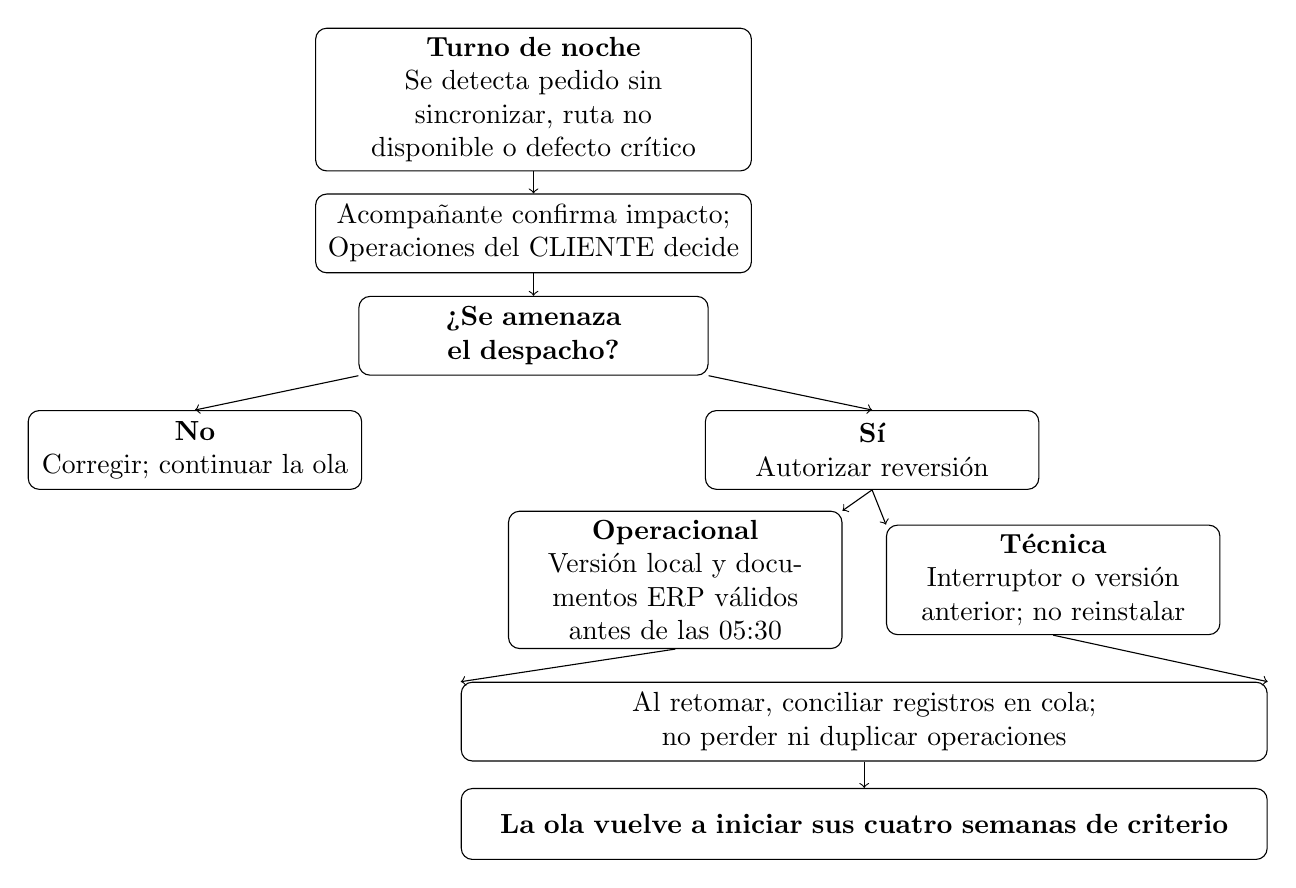
\begin{tikzpicture}[font=\LFXcuerpofigura]
    \node[draw,rounded corners,align=center,text width=5.3cm,minimum height=11mm]
      (detect) at (0,0)
      {\textbf{Turno de noche}\\Se detecta pedido sin sincronizar, ruta no disponible o defecto crítico};
    \node[draw,rounded corners,align=center,text width=5.3cm,minimum height=10mm]
      (verify) at (0,-1.7)
      {Acompañante confirma impacto; Operaciones del CLIENTE decide};
    \node[draw,rounded corners,align=center,text width=4.2cm,minimum height=10mm]
      (decision) at (0,-3.0)
      {\textbf{¿Se amenaza el despacho?}};
    \node[draw,rounded corners,align=center,text width=4cm,minimum height=10mm]
      (continue) at (-4.3,-4.45)
      {\textbf{No}\\Corregir; continuar la ola};
    \node[draw,rounded corners,align=center,text width=4cm,minimum height=10mm]
      (authorize) at (4.3,-4.45)
      {\textbf{Sí}\\Autorizar reversión};
    \draw[->] (detect) -- (verify);
    \draw[->] (verify) -- (decision);
    \draw[->] (decision.south west) -- (continue.north);
    \draw[->] (decision.south east) -- (authorize.north);
    \node[draw,rounded corners,align=center,text width=4cm,minimum height=12mm]
      (operational) at (1.8,-6.1)
      {\textbf{Operacional}\\Versión local y documentos ERP válidos antes de las 05:30};
    \node[draw,rounded corners,align=center,text width=4cm,minimum height=12mm]
      (technical) at (6.6,-6.1)
      {\textbf{Técnica}\\Interruptor o versión anterior; no reinstalar};
    \draw[->] (authorize.south) -- (operational.north east);
    \draw[->] (authorize.south) -- (technical.north west);
    \node[draw,rounded corners,align=center,text width=10cm,minimum height=10mm]
      (reconcile) at (4.2,-7.9)
      {Al retomar, conciliar registros en cola; no perder ni duplicar operaciones};
    \draw[->] (operational.south) -- (reconcile.north west);
    \draw[->] (technical.south) -- (reconcile.north east);
    \node[draw,rounded corners,align=center,text width=10cm,minimum height=9mm]
      (restart) at (4.2,-9.2)
      {\textbf{La ola vuelve a iniciar sus cuatro semanas de criterio}};
    \draw[->] (reconcile) -- (restart);
  \end{tikzpicture}
  \caption{Procedimiento de reversión de la Etapa 1. Fuente: elaboración propia a partir del Capítulo 3, sección 3.4.4, y del paquete 4.1.2.}
  \label{fig:T18-reversion}
\end{figure}

El procedimiento debe conservar información: los registros capturados quedan en cola y se concilian al retomar; su integridad se verifica en el ensayo. Lo que se pierde es la jornada de operación en la solución nueva para esa ola, que vuelve a empezar su período de cuatro semanas (Capítulo 3, sección 3.4.4; paquete 4.1.2; Caso 02, sección 17.6, punto 4). El tiempo de cada nivel de reversión se mide en el ensayo en Preproducción que precede a cada corte (RT-20.02).

\subsection{Acompañamiento en terreno y estabilización}

Después de cada paso a producción hay cuatro semanas de estabilización por ola, el mismo período que exige el criterio de avance. La dotación se deriva de la operación del caso (Capítulo 3, sección 3.4.4; paquete 4.2.2), como muestra la Tabla \ref{tab:T18-dotacion}.

\parte{tablas/tab_T18_dotacion}

Si la ola cubre solo una zona, la dotación de calle se reduce en proporción a sus rutas, y la dotación decrece según la curva de adopción, como exige el RT-20.05.

\subsection{Capacitación y certificación}

La capacitación se hace en el puesto y en la ruta, sin detener la venta ni el reparto (Caso 02, sección 13.3, condición 5). Usa las cuatro modalidades del Art. 90.2: presencial en cada sitio, en línea sincrónica, autoformación en línea y acompañamiento en el puesto durante la marcha blanca. Cada perfil se certifica antes de cerrar la marcha blanca, porque el Art. 17.3 exige personal «capacitado y certificado conforme al plan de capacitación aprobado» (paquetes 7.1.1 a 7.1.6 y 7.3.1). Los usuarios administradores y el equipo técnico del CLIENTE se certifican además conforme al Art. 90.4. La Tabla \ref{tab:T18-perfiles} presenta los perfiles operativos.

\parte{tablas/tab_T18_perfiles}

Los conductores de transportistas no son trabajadores de la compañía. Su incorporación requiere el acuerdo operacional firmado con cada una de las diez empresas (paquete 5.4.1), y una ola de reparto no incluye a una empresa transportista hasta que su acuerdo esté firmado (Capítulo 3, Anexo 3.I; Caso 02, sección 13.3, condición 6). El uso del GPS para control de jornada requiere el acuerdo previo con el sindicato (paquete 5.4.2; S-13).

\subsection{Medición de la adopción}

La adopción se mide por perfil y por ola con los indicadores del Capítulo 3, Anexo 3.I: pedidos capturados en la aplicación sobre el total, entregas con prueba digital, preparadores certificados por turno y conductores con autenticación válida. La meta es que el 100 \% de los usuarios de la ola esté certificado y que el 100 \% de las transacciones de la ola se registre en la solución al retirar el papel. Si una ola no alcanza la meta, no avanza y se extiende el acompañamiento (paquete 7.2.5).

La respuesta es distinta según el grupo (Caso 02, sección 17.6, punto 7). El personal con 20 o 30 años en la compañía recibe acompañamiento individual en su puesto o ruta y reconocimiento formal de su conocimiento (paquete 7.2.1), y el personal rotativo de preparación cuenta con un tutor por turno y certificación en el puesto (paquete 7.1.2).

\subsection{Cierre de la marcha blanca y paso a producción}

La marcha blanca de la Etapa 1 cierra cuando se cumplen a la vez las seis condiciones del Art. 17.3. El paso a producción ocurre en el mes 16, fuera de las fechas prohibidas, y se formaliza con el acta del H7 (paquete 4.2.3). Si al término del mes 15 no se cumplen las condiciones, la marcha blanca se extiende a costo del adjudicatario, sin mover las fechas de las fases siguientes (Art. 17.3).

\section{Etapa 2: marcha blanca de los meses 19 y 20 y producción desde el mes 21}

La Etapa 2 se implanta sobre la plataforma ya estabilizada de la Etapa 1, con una marcha blanca más corta y en convivencia con la Etapa 1 en producción.

\subsection{Alcance y despliegue}

La Etapa 2 pone en producción el intercambio electrónico de pedidos y avisos de despacho con las cadenas (M11 Canal moderno), el portal de clientes, el portal de transportistas y el costo de servir por cliente y por entrega (M10). Corresponde a los paquetes 3.5.1 a 3.5.4, 3.6.5 y 3.6.6 del Formulario T-14 y se despliega sobre la plataforma de la Etapa 1, sin rehacer su arquitectura (Bases Administrativas, Art. 15.1).

El despliegue avanza por cadena y por grupo de usuarios. Cada cadena se incorpora al intercambio electrónico cuando su perfil está certificado (paquetes 3.6.5 y 3.6.6) y, hasta entonces, sus pedidos siguen con carga manual controlada, que no acredita el resultado R18-13. Los portales se habilitan por grupo de clientes y por transportista, y el costo de servir se habilita para Comercial y Finanzas con los hechos acumulados desde la marcha blanca de la Etapa 1.

La marcha blanca E2 ocupa meses 19–20. Todo el alcance requerido de cadenas, portales y costo de servir debe activarse antes de F − 28 días; una cadena todavía no certificada no se excluye del denominador de aceptación. La operación registra el 100 \% de sus pedidos y entregas reales, con los perfiles certificados y la conciliación requerida. La conversión promedio de dos meses a 8,7 semanas no determina una fecha límite contractual.

En el escenario ilustrativo de inicio en febrero de 2027 (Anexo 7.A del Subdocumento 7), el mes 19 cae en agosto de 2028 y el mes 20 en septiembre, lo que tiene tres consecuencias. La primera es que toda habilitación de la Etapa 2 ocurre en agosto, porque el congelamiento total va del 1 al 25 de septiembre (Caso 02, RT-10.05), además de respetar F − 28 días y los primeros tres días hábiles de agosto. La segunda es que la evidencia de cierre atraviesa septiembre: incluye el volumen real de cada día y el peak cuando ocurre, con pruebas previas a 1,5 veces la carga peak. Este sería el primer septiembre de E1 en producción, por lo que la preparación de continuidad de ambas etapas es crítica. La tercera es que entre el 1 y el 25 de septiembre no se despliega ningún cambio sobre ninguna de las dos etapas: ante un defecto de la Etapa 2, se aplica la contingencia aprobada conforme a la sección 6.4, sin presumir que un cambio de configuración está exento del congelamiento.

La capacidad para ese peak se demuestra antes del H11 con las pruebas de carga a 1,5 veces el peak, con ambas etapas activas (paquete 3.9.3). El caso advierte que septiembre es «el período de mayor exigencia sobre cualquier componente nuevo» (sección 13.2).

\subsection{Pruebas previas}

Antes del paso a producción del mes 21 se aprueban las mismas pruebas de la sección 2.2, aplicadas a la Etapa 2 (paquetes 3.9.1 a 3.9.7). Se agrega una exigencia: demostrar que la Etapa 1, ya en producción, no se degrada. Las pruebas de carga se ejecutan con ambas etapas activas (3.9.3), y la recuperación ante desastres, con ambas etapas (3.9.4).

\subsection{Indicadores diarios y umbrales de cierre}

Se aplican los indicadores de la sección 2.4 a los usuarios y transacciones de la Etapa 2, más los propios de su alcance, que presenta la Tabla \ref{tab:T18-ind2}.

\parte{tablas/tab_T18_ind2}

Los dos últimos indicadores protegen a la Etapa 1 durante la convivencia. R18-11 se acepta con la reconciliación con la contabilidad del mes (Capítulo 3, Anexo 3.J).

\subsection{Reversión}

La reversión de la Etapa 2 no toca la Etapa 1. Desactiva mediante un indicador de funcionalidad la capacidad de la Etapa 2 que falla, y la operación vuelve al procedimiento anterior de esa capacidad: carga manual controlada de los pedidos de la cadena, atención asistida a clientes y transportistas, o el cálculo vigente de costos. Estos procedimientos sostienen contingencia auxiliar y no acreditan R18-13 ni habilitan cierre mientras una capacidad requerida esté desactivada. Ningún despliegue ni reversión ocurre en la ventana de 05:30 a 07:00 ni en fechas prohibidas (paquete 4.1.3).

\subsection{Estabilización, capacitación y certificación}

Después del paso a producción del mes 21 hay cuatro semanas de estabilización, concentrada en los usuarios nuevos: Comercial, Finanzas, las cadenas y los transportistas (paquete 4.3.2). Comercial y Finanzas se certifican en costo de servir antes del cierre de la marcha blanca (paquete 7.3.2), y la gestión del cambio con las cadenas y los transportistas se hace con el paquete 7.2.2.

\subsection{Cierre y aceptación final}

La marcha blanca de la Etapa 2 cierra con las seis condiciones del Art. 17.3. El paso a producción del mes 21 es la aceptación final de la implementación (H12, paquete 4.3.3), condicionada a la constitución de la garantía de correcto funcionamiento (paquete 4.3.4; Bases Administrativas, Art. 37.1).

\section{Convivencia entre la Etapa 1 y la Etapa 2}

La convivencia sigue las reglas del Art. 17.2. En los meses 13 a 15 coexisten la marcha blanca de la Etapa 1 y el desarrollo de la Etapa 2: el desarrollo de la Etapa 2 no despliega en Producción ni modifica las funciones de la Etapa 1 en marcha blanca, y los frentes de ambos esfuerzos están en el Formulario T-15. En los meses 19 y 20 la Etapa 1 está en producción y la Etapa 2 en marcha blanca, con una única fuente de verdad para los datos compartidos (pedidos, clientes, guías y entregas): la Etapa 2 lee y extiende los registros de la Etapa 1, sin copiarlos ni volver a digitarlos. En el mes 21, el paso a producción de la Etapa 2 no degrada la disponibilidad, el desempeño ni la integridad de los datos de la Etapa 1, y la Operación comienza ese mes con ambos alcances. La Figura \ref{fig:T18-convivencia} muestra el flujo de datos de los meses 19 y 20.

\begin{figure}[htbp]
  \centering
  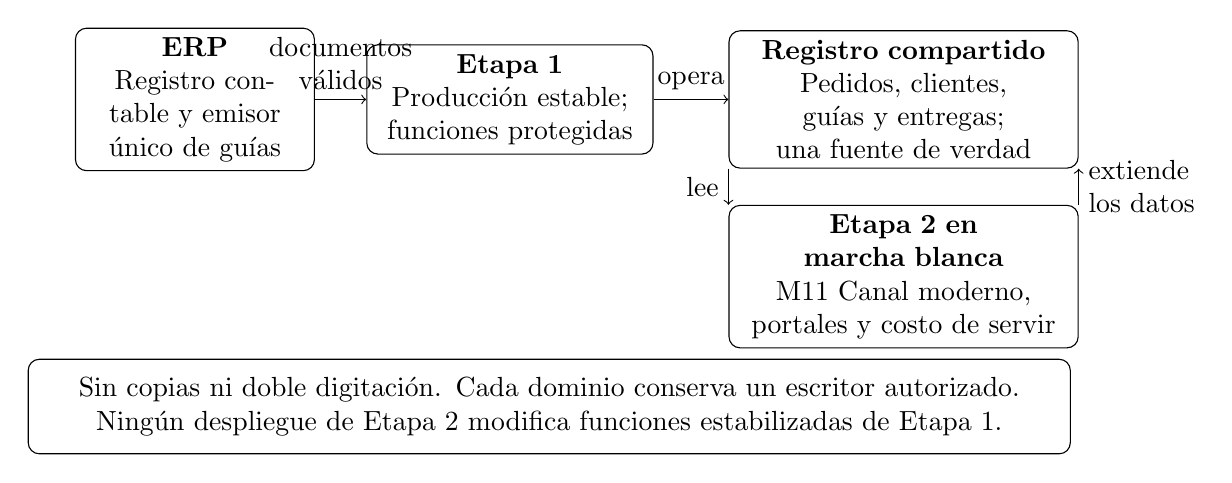
\begin{tikzpicture}[font=\LFXcuerpofigura]
    \node[draw,rounded corners,align=center,text width=2.8cm,minimum height=13mm]
      (erp) at (0,0)
      {\textbf{ERP}\\Registro contable y emisor único de guías};
    \node[draw,rounded corners,align=center,text width=3.4cm,minimum height=13mm]
      (stage1) at (4,0)
      {\textbf{Etapa 1}\\Producción estable; funciones protegidas};
    \node[draw,rounded corners,align=center,text width=4.2cm,minimum height=15mm]
      (shared) at (9,0)
      {\textbf{Registro compartido}\\Pedidos, clientes, guías y entregas; una fuente de verdad};
    \node[draw,rounded corners,align=center,text width=4.2cm,minimum height=15mm]
      (stage2) at (9,-2.25)
      {\textbf{Etapa 2 en marcha blanca}\\M11 Canal moderno, portales y costo de servir};
    \draw[->] (erp) -- node[above,align=center]{documentos\\válidos} (stage1);
    \draw[->] (stage1) -- node[above,align=center]{opera} (shared);
    \draw[->] (shared.south west) -- node[left,align=right]{lee} (stage2.north west);
    \draw[->] (stage2.north east) -- node[right,align=left]{extiende\\los datos} (shared.south east);
    \node[draw,rounded corners,align=center,text width=13cm,minimum height=12mm]
      at (4.5,-3.9)
      {Sin copias ni doble digitación. Cada dominio conserva un escritor autorizado.\\
       Ningún despliegue de Etapa 2 modifica funciones estabilizadas de Etapa 1.};
  \end{tikzpicture}
  \caption{Convivencia de la Etapa 1 en producción con la Etapa 2 en marcha blanca. Fuente: elaboración propia a partir de la arquitectura lógica del Capítulo 4.}
  \label{fig:T18-convivencia}
\end{figure}

La Etapa 1 escribe en el registro único y la Etapa 2 lo lee y lo extiende; ninguna de las dos mantiene una copia de los datos de la otra, por lo que no existe una doble digitación que conciliar.

\section{Transferencia a la Operación}

La transferencia al equipo de TI de cuatro personas del CLIENTE se hace antes del mes 21. Comprende los procedimientos de operación documentados y ensayados y la base de conocimiento (paquetes 7.1.4 y 3.11.2). Sigue una mentoría de seis meses después del paso a producción de la Etapa 2 (paquete 8.5.2; RT-22.07).

Queda como servicio permanente del adjudicatario durante los 36 meses lo que el Capítulo 3, sección 3.4.5, asigna a LafroX: el centro de operaciones, la mesa de servicio, la gestión de incidentes, la continuidad, la seguridad y el mantenimiento, que corresponden a los paquetes 8.1 y 8.2 (Caso 02, sección 17.6, punto 8).

\section{Condiciones de programación, recursos y continuidad}

Los criterios siguientes gobiernan la programación bajo supuestos explícitos y prevalecen sobre descripciones gráficas históricas. La aceptación contractual exige actas y evidencias, no la sola descripción de estos controles.

\subsection{Alcance completo de las olas y orden de incorporación}

Las olas incorporan todo el alcance de cada etapa en el orden siguiente.

\parte{tablas/tab_T18_olas_alcance}

Las semanas son relativas a H6 y son supuestos de preparación; al confirmar fechas se convierten a días permitidos. El piloto en Talca facilita probar la integración con WMS/ERP, pero no se presume aprobado. No se inventa un número de zonas: el plan de rutas vigente del CLIENTE define los grupos y su volumen. El responsable de Operaciones y el Líder de Implantación registran sitio, rutas, módulos, usuarios, escritor autorizado y fecha de activación en el acta de cada grupo. Si un grupo no está listo, no se sustituye su volumen por una muestra para acreditar cierre.

Los dominios pueden habilitarse en paralelo sin intervenir simultáneamente el mismo proceso/sitio ni crear doble escritura. Una recepción habilitada alimenta bodega con conciliación diaria, mientras se acumula su evidencia; el retiro del respaldo exige cuatro semanas consecutivas por grupo. El último grupo se propone en semana 8 y nunca después de F − 28 días. Con apertura del período de H6 el 1 de febrero de 2028, sin activar cambios durante los primeros tres días hábiles, y cierre al comenzar el 1 de mayo de 2028, la evidencia comprende 3–30 de abril; todos los grupos deben estar operativos antes del 3 de abril. La semana 8 cae dentro de marzo y evita depender de la semana 9 de abril. Es un ejemplo calendario, no una fecha aprobada: el calendario hábil del CLIENTE y las fechas efectivas determinan las activaciones. H7/\allowbreak{}H12 respetan también los primeros tres días hábiles de su mes; la continuidad y evidencia se mantienen hasta el acta, sin usar esa espera para recortar la marcha blanca.

El costo de servir de M10 Analítica se reserva a E2; sus indicadores operacionales pertenecen a E1. M9 Calidad y trazabilidad y M12 Telemetría se activan desde la primera ola y amplían cobertura conforme al proceso.

\subsection{Orden de cadenas, portales y cierre E2}

En el mes 18 se congela el registro de cadenas y perfiles de intercambio con Operaciones/Comercial; 3.6.5 y 3.6.6 deben tener pruebas de conformidad antes de activar cada cadena. El orden propuesto es: perfiles ya certificados y accesos disponibles primero; perfiles con mayor variación o dependencia externa después, todos dentro del mes 19 y antes del inicio de las cuatro semanas finales. No se inventan nombres ni cantidades de cadenas.

Portales por grupo de usuarios y costo de servir avanzan en paralelo en dominios distintos. El acta registra el 100 \% del alcance de cadenas exigible, no sólo las que lograron certificarse. Si una cadena requerida falta, R18-13 permanece incumplido; la carga manual es contingencia y no acredita intercambio electrónico. La habilitación termina antes de septiembre bajo el calendario supuesto y antes de la fecha efectiva que permita cuatro semanas de cierre; no se usa «4,7 semanas» como fecha límite exacta.

\subsection{Dotación, estabilización y soporte entre etapas}

Se mantiene el mínimo simultáneo de 13 puestos de acompañamiento derivado del SD3: dos en CD, tres en plataformas, siete en ruta y uno de coordinación. Puestos y personas de relevo son conceptos distintos. Para planificar cuatro semanas (24 días operativos), se asumen ocho horas por jornada de terreno: 12 \ensuremath{\times} 24 \ensuremath{\times} 8 + 160 de coordinación = 2.464 HH; los relevos se dimensionan con 128 HH efectivas/persona-mes en T-15. No se supone que dos personas solas cubran todos los turnos nocturnos del mes.

\parte{tablas/tab_T18_prevision}

Las previsiones mensuales son una curva inicial, no una retirada automática. El JP y Operaciones autorizan cada decremento en un acta con indicadores diarios y cobertura por perfil; si falla un indicador, se retiene o restituye el nivel anterior sin desplazar hitos. Toda extensión requiere recalcular HH, relevos y capacidad disponible del T-15. Para E2 se prevén cuatro semanas de atención reforzada; después se integra a F8 si la Contraparte Técnica confirma estabilidad.

Desde H7 y hasta el mes 20, el paquete 4.2.2 incluye soporte puente: NOC 24\ensuremath{\times}7, mesa 04:00–22:00 de lunes a sábado y 24\ensuremath{\times}7 en septiembre/diciembre, especialistas para críticos/altos 24\ensuremath{\times}7 y escalamiento operativo. El T-15 separa cobertura y reserva de correcciones de acompañamiento. En el mes 21 se transfiere a 8.1.1/\allowbreak{}8.1.2 sin brecha de atención. Los responsables de incidentes, escalamiento y datos son los mismos en ambas etapas; E2 no dispone de un segundo escritor de los datos E1.

\subsection{Tiempo de reversión y ensayo de capacidad}

Objetivos propuestos para el ensayo previo a cada corte: nivel técnico \ensuremath{\leq}10 minutos; preparación de contingencia operacional \ensuremath{\leq}30 minutos en paralelo; verificación y autorización de despacho \ensuremath{\leq}10 minutos adicionales. Tiempo total objetivo = máximo(10,30) + 10 = 40 minutos. Decisión límite propuesta 04:45; restauración operacional objetivo 05:25, con cinco minutos antes de las 05:30. Son los objetivos que el ensayo mide antes de cada corte en Preproducción. El tiempo de restauración de incidentes críticos \ensuremath{\leq}4 horas del Art. 78.3 es una métrica mensual de operación distinta de estos objetivos de reversión.

El ensayo de 4.1.2 registra detección, decisión, comienzo/fin técnico, disponibilidad de la versión local, conciliación mínima, guías emitidas por ERP, disponibilidad de rutas y autorización del CLIENTE. Debe demostrar el flujo completo de los 96 despachos y las integraciones fallidas, sin pérdida/duplicación ni emisión tributaria por un sistema no autorizado. Si no termina antes de las 05:30 o no acredita ese volumen, el corte no se autoriza y se activa el riesgo R8-01 del Subdocumento 8. La falla del ERP requiere su contingencia tributaria aprobada; disponer de papel no prueba que se puedan emitir DTE ni cumplir el despacho.

WMS permanece en solo lectura como respaldo de consulta conforme a S-14: no se reactiva su escritura para revertir. La vuelta operacional mantiene o restituye una versión local probada, único escritor y documentos válidos del ERP; conserva UUID/colas para conciliar. El papel y la carga asistida sólo sostienen tareas auxiliares y no reemplazan el despacho de 96 camiones. Ante cualquier evidencia de pérdida o duplicación se bloquea la aceptación; la conservación se comprueba, no se presume.

Durante congelamientos, se aplica la continuidad previamente autorizada por el CLIENTE. Los indicadores de funcionalidad están sujetos a las prohibiciones de cambio. Si deshabilitar una función modifica producción, su ejecución requiere el procedimiento de emergencia acordado y la autoridad correspondiente. La reversión no puede degradar E1 ni crear doble digitación. Fuera de emergencia, las habilitaciones, cortes y cambios respetan todas las fechas y ventanas prohibidas.

\subsection{Controles nuevos de coordinación y aceptación}

Los paquetes 3.3.6, 3.4.2 y 3.4.6 incluyen la coordinación de reserva y retención (SD4, apartado 4.1.4.4 y Anexo 4-G): retención local por lote/ubicación, acuse durable antes de confirmar pedido, UUID e idempotencia y época de autoridad. 3.8.1/\allowbreak{}3.8.3 incluyen AL-STOCK-01 y AL-ACT-01 con corte, reintento, concurrencia y ausencia de doble descuento o retención duplicada. El dimensionamiento se recoge en el Anexo 4-I, Tabla A.10, y el Anexo 4-W, Tablas A.32 y A.33: 46.968 mensajes/día normales y 87.228 en peak, con un máximo de cuatro mensajes por línea. La retención consumida no se libera, por lo que esa holgura cubre líneas repartidas entre lotes o sitios. AL-STOCK-01 mide la proporción de líneas con más de una retención y 3.8.4/\allowbreak{}3.9.3 verifican la carga y el drenaje, sin sumar la coordinación al drenaje tras un corte (4-W.5).

El RPO \ensuremath{\leq}15 min se cumple con fibra, LTE y Starlink. La falla simultánea de los tres caminos seguida de la destrucción del sitio antes de reponer alguno es el riesgo residual declarado en SD4 4.3.2.4 (RT-02.11), gestionado en SD8 con R8-05. AL-DR-01 verifica las alarmas de retraso a 5 y 15 min, la reposición del enlace, la preemisión de guías y el NAS WORM, y mide el RPO y el RTO en conmutación real antes del H5 y del H10.

\section{Referencias}

Las Bases se citan con su documento y el artículo, capítulo, sección o código del requisito.

\begin{itemize}
\item Distribuidora Puelche S.A. (2026a). \emph{Bases Administrativas de Licitación N.º TFEP-01/\allowbreak{}2026: Contratación de Solución Integral de Software y Servicios de Operación}.

\item Distribuidora Puelche S.A. (2026b). \emph{Bases Técnicas Transversales de Licitación N.º TFEP-01/\allowbreak{}2026}.

\item Distribuidora Puelche S.A. (2026c). \emph{Caso 02: Logística. Especificaciones del problema y operación de Distribuidora Puelche S.A.}

\end{itemize}
\section{Declaración de uso de IA}

En cumplimiento de la sección 7.2 de las Aclaraciones de la licitación, la tabla siguiente declara el uso de herramientas de inteligencia artificial en este formulario, con la revisión humana de cada parte. La declaración se consolida en el Formulario A-6.

\parte{tablas/tab_T18_IA}

